Machine Learning has emerged as booming field in Computer Science that provides a lot of opportunities for innovation and growth.
The important thing to know about machine learning is what is in the name: teaching machines to learn.
Through various approaches and algorithms it is possible to feed these machines input data and coach them to predict outcome events without being explicitly programmed to do so [\cite{hansen1990neural}].
Machine Learning algorithms come with a caveat though that unfortunately this research exhibits, and that is that effective machine learning is difficult because finding patterns is hard and often there isn't enough training data available to effectively train the algorithm to make predictions.
The data here is large but rather minute compared to the large amounts of data normally used to train such learning algorithms.
As such, the results achieved here aren't as strong as one would hope but this research establishes an approach that could be expanded and fed more data to achieve a more effective result.

Machine Learning can refer to many different topics as it is a broad field, but in this research the learning algorithms used were Neural Network, Naive Bayes Classifer, and Decision Tree.
All of these fall into the supervised learning category of machine learning wherein a training set of data is input, along with the target outcome that allows the models to use this data and output target to learn how to predict the outcome [\cite{dietterich1998approximate}].
Before the learning algorithms are discussed more in-depth it is important to understand the data that was produced to create the learning set and how it was used.

\section{Topic Classifier Sets}
An important part of the latter half of the preprocessing work for this research was the topic classifier sets.
At first, the sentiment score was calculated for each presidential address with an overall score from -1 to 1, indicating their tone when delivering that address.
After these were calculated, they were analyzed to look for trends in each president's tone to see if there were any interesting patterns.
As an additional breakdown to see if there was any more context-specific information that could help determine a president's political party, topic categories were added to diversify the scores of the presidents.

Four Presidential Addresses were chosen (Washington, Lincoln, Kennedy, Obama) and manually read to discover what words were being used when talking about certain general topics within the United States.
The twelve topics that were identified were: crime, economy, education, energy, environment, family, foreign affairs, government, job, religion, terrorism, and war.
Text files were created using the trigger words that were collected for each major topic.
The trigger words were pulled from the four addresses mentioned above and from various other addresses as they were skimmed through.
During the algorithm, these text files are converted into arrays and as a sentence is being processed, it is scanned for these trigger words and if it has one of those words then it assigned to that topic.
Then the sentiment analysis is conducted on each of the sentences within each of the categories to obtain a topic sentiment score for each President.
The implementation of this part of the algorithm can be seen in Algorithm \ref{alg:classification} on the next page, and the trigger words are used starting on line \ref{alg:classification:topic}.

This processing was conducted on every address and the sentiment score for each topic was found for each President, which resulted in a vector for each address that had their overall sentiment score and the sentiment score for each topic covered in the address.
These scores for each address were then averaged together to create an overall vector for each president that could be used for classification and learning to learn their political party.
This vector consisted of 15 values (the President's name, the overall sentiment score, 12 of the topic sentiment scores mentioned above, and the President's political party) to be used for learning.
For example, George Bush's vector was ['Bush', 0.1340853948691, 0.1302164475371004, 0.13079766376531318, 0.13296404930509467, 0.13296404930509467, 0.13743239837292998, 0.13949090904366207, 0.14036831555702362, 0.1434021113795079, 0.14341784426710505, 0.14306495549111073, 0.14278963481416337, 0.14030583896785492, 'Republican'].

\begin{singlespace}
\begin{algorithm}[H]
\DontPrintSemicolon
\KwIn{All State of the Union Addresses}
\KwOut{The sentiment score for each Presidential Address for each category.}
\BlankLine
open all .txt files and store them in lists of special category trigger words\;
\For{each address in the State of the Union Addresses}
	{format address\;
	split address in to sentences\;
	\For{each sentence in the address}
		{add sentence to 'overall' category\;
		\If{sentence contains category trigger word \label{alg:classification:topic}} 
		{add sentence to category}
	\For{each category}
		{append list of sentences for that category to an overall list}
	\For{each topic in the overall list}
		{\For{each word in the topic}
			{create word count for each word and store it in a dictionary\;
			\If{previous word negator}
				{increment negator counter for that word by one}
			\If{previous word intensifier}
				{increment intensifier counter for that word by one}
			}
		\For{each word in the dictionary}
		{\If{word is in lexicon}
		{\If{length of negators[word] != 0}
		{Subtract length from total count for that word}
		}
		\If{length of intensifiers[word] != 0}
		{Raise length number of scores to the power of 2}
		Calculate the Sentiment Score by multiplying the number of occurrences of the term by the score in the lexicon.
		}
		}
	}
	}
	
\caption{Sentiment Analysis Algorithm}
\label{alg:classification}
\end{algorithm}
\end{singlespace}

\section{Normalization}
As an added measure to clearly show the differences between different vectors, each of the values was normalized from -1 to 1 using a simple normalization algorithm.
This normalization process aided in distinguishing the minute differences that manifest themselves when the data is more spread out on a greater range.
The normalization method can be seen in Algorithm \ref{alg:two}.

\begin{singlespace}
\begin{algorithm}[H]
\DontPrintSemicolon
\KwIn{Master array (an array of all the Presidential vectors)}
\KwOut{The Master array (Now with all values normalized)}
\BlankLine
\For{array in master}
	{old\ min = min(array)\;
	old\ range = max(array) - old\ min\;
    	new\ min = -1\;
   	new\ range = 2\;
    	array \= [float((n - old\_min) / old\ range * new\ range + new\ min) for n in array]\;
	new\_\ master.append(array)}
\caption{Normalization Algorithm}
\label{alg:two}
\end{algorithm}
\end{singlespace}

\section{Neural Networks}
Neural Networks take their name because they are trying to mimic and that is of a human's brain and its biological neural networks that allow it to make decisions [\cite{hansen1990neural}].
This concept was mirrored and used to produce neural networks that are fed input data that is labeled as either exhibiting a behavior or not exhibiting a behavior and using that data to predict the unknown label of future inputs.
The neural network has no inherent knowledge about the sentiment scores inserted into them, nor the political party label but it merely uses this data to learn patterns and uses these patterns to predict the political party of an unknown president using their sentiment scores.
This first step of learning from data that is labeled is called the training phase.
The training phase is important since the effectiveness of the algorithm relies entirely on the algorithm being trained correctly and effectively [\cite{hepner1990artificial}].
The goal is to have a diverse set of inputs to give the algorithm a range of data, and then tell it how many times to repeat over the data to learn it.
Finding the sweet spot of how many repetitions to utilize when having the algorithm learn the input data is very important, as too many repetitions causes the algorithm to confine itself to just the input data and it will lose the ability to generalize patterns to predict outcomes correctly, and too few repetitions prevents the algorithm from interacting with the data enough to draw meaningful patterns and conclusions from it.

A visualization for how a neural network works can be seen in Figure \ref{fig:nndiagram} [\cite{juan2013nndiagram}].


\begin{figure}
\begin{center}
  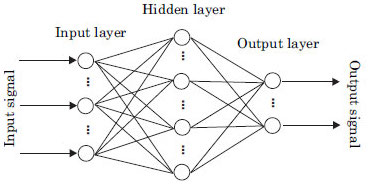
\includegraphics[width=250pt]{images/nndiagram.jpg}
  \caption{Neural Network Diagram}
  \label{fig:nndiagram}
  \end{center}
\end{figure}



\section{Naive Bayes Classifier}
A Naive Bayes classifier functions in a very similar fashion to that of a neural network but it is less of a black box approach and more of a statistical approach.
Using the input and target data, the Naive Bayes classifier uses a statistical model to predict values rather than strictly pattern recognition [\cite{murphy2006naive}].
Naive Bayes has actually been discovered to handle small amounts of data better than neural networks so it was important to add here since both have their strong suits in predicting values.
Naive Bayes is a much simpler algorithm which can limit its performance and effectiveness as it attempts to fit its training data too closely, causing it to lose accuracy, whereas a neural network's complexity can actually overfit the data, which makes it weaker at predicting data outside the input data set.

\section{Decision Tree Classifier}
A Decision Tree Classifier functions in almost the exact same way that Naive Bayes does, but instead of predicting one output value, a decision tree examines the data to find steps it could take to make the correct prediction.
Using these steps, a Decision Tree produces a list of steps it iterates through for each value and uses the outcome of each of the steps to predict the output value.
This is effective with data that shows more trends and is sufficiently spread out, but this function struggled with this data as the decisions it made weren't clear and it overfit itself to the data which caused performance issues in this research [\cite{dietterich1995overfitting}].
A Decision Tree can be useful since it produces a model in a human readable fashion that gives insight into how it makes a prediction, which can allow for easier fine-tuning of the data and the algorithm to produce the best results.
Much of machine learning can be a black box approach and this insight in to the inner workings of this algorithm simplifies it, but also limits it as this simplicity makes the algorithm not always as effective in its predictions.

\section{Leave-one-out Cross-validation}
In order to evaluate the effectiveness of the algorithm, leave-one-out cross-validation was used.
This validation method works by iterating over the data and hiding one of the points of data and uses the remaining data points to predict the hidden one [\cite{tzutsung2015validation}].
This is then repeated for each of the data points to be the hidden one.
In this research, each address is represented as a vector of 13 numbers and two strings, indicating the sentiment scores for each category as well as the overall score and the final value is the political party the president belongs to.
Then, using these vectors, one of them is hidden, and the rest of the vectors are used to predict the values for the hidden vector.
This process is then repeated for each of the vectors until all of them have been the hidden one and had their output predicted.
This validation method ensures the algorithm is working properly and can properly predict a set of values using the existing data set.

\section{Results}
The results from the machine learning algorithms were less than stellar but provide interesting insight into the problems at hand regardless of this.
The breakdown of Democrat and Republican is 38\% and 62\% respectively.
So, ideally the desired accuracy for an effective learning algorithm would be reasonably above 62\% as you could successfully get 62\% every time by predicting Republican for every single president.
Unfortunately, the results achieved for these machine learning algorithms were 59.5\% for the Neural Network and 35.71\% for the Naive Bayes Classifier and Decision Tree.
These accuracy numbers are less than satisfactory but there is much to say about the data being handled and how effective translating qualitative into quantitative data works.
Text data at its heart is qualitative data since there is feeling and tone and intangible elements of speech that one can't quite quantify just yet but there is a way to do it.
This research ran into many of these same roadblocks that come with translating text data into numeric data as some of this intangible meaning is lost and has to be reproduced mechanically to reach necessary conclusions about the data.

These results are less than astounding but it is interesting how much better the neural network performed than the statistical measure of the Naive Bayes.
So the patterns drawn from the neural network were stronger indicators of party alliance and even though the data source was small, the neural network performed stronger even though typically the opposite is the case when comparing these two approaches as was mentioned previously.
The Decision Tree Classifier has the same accuracy as the Naive Bayes as they both function similarly when the data set is small and they function very similarly in this research.
Instead of creating a pattern to discern the vector values for each presidential party, the decision tree shows that it assigned the sentiment scores value to that category and if the values matched another one, it would look at the party of the matched one and assign it that, all the way down the list of categories.
This overfitting caused the algorithm to focus too much on early results and not look at the whole data set before predicting a value which caused it to have an interestingly low prediction accuracy rate, worse than picking every party the same [\cite{dietterich1995overfitting}].
The concept and algorithms themselves are interesting but the accuracy and results are less than convincing about whether this can adequately be proven as a relation.

\subsection{Vector Analysis}
To add more context to the vector creation, here are two vectors from the calculations that will be interpreted.
The two vectors can be seen in Table \ref{table:vector} below, and a full list of all of the vectors can found in the appendix [Here - To be completed].

The two excerpts are a small portion of the data collected but they both show interesting trends in tone across the different topics.
Also, to be noted is the fact this these numbers are an average for all of the addresses given by the President and not single term.
This is especially pertinent since George Bush had an extremely low sentiment score on his address immediately after 9/11 but his other ones were generally higher and averaged him out to a more positive sentiment score.
Overall and across the categories, Abraham Lincoln has lower sentiment scores than Bush and actually his overall sentiment score is fairly higher than any one of his topic scores.
This indicates a topic not featured here that he had an overwhelmingly positive tone on that averaged his overall score higher, or just a general positive mood not directed towards any specific topic.

Abraham Lincoln's presidency spanned the length of the Civil War so his tone during these State of the Union addresses can be viewed as the presidential perspective during this national outbreak of war.
Lincoln does have a lower tone score than other presidents but it isn't as low as one might expect considering the events that were transpiring.
This might indicate a generally positive tone as Lincoln tries to unify the country, but also follows the trend of Presidents having a generally more positive tone on their addresses overall.
Also the tone on war is lower but also isn't out of line with any of the other categories really and this calls into question the exact calculations that go in to producing these scores.
War can be a difficult topic to nail down in terms of meaning as most mentions of war play in to its destructive capabilities so trying to separate and distinguish positive and negative tone surrounding war can be difficult.
This might play in to the numbers seen here and how they are generally close together since the trigger words and way the categories are sorted might need work to more effectively reflect the tone on specific topics.

Much of the same can be said for George Bush's vector with a few interesting differences.
Bush's scores deviate below and above his sentiment score, with stronger positive sentiment occurring in Family and Religion, and lower scores in Economy and Government.
George Bush was a Conservative and a large proponent of family values and was a devout Christian so the positive tone coming from those categories is not surprising.
The lower scores for economy and war also make sense given the times as the economy was in a downturn at the latter half of his presidency and the Iraq war was going on during his presidency.
This war sentiment score is deceiving, as was mentioned before, in how war is normally discussed, which should be considered.

It is interesting how the trend for war was equivalent for both presidents, being lower than the overall sentiment score.
And George Bush had the reverse issue from Lincoln, where Bush's individual topic scores are all mostly greater than his overall score, possibly showing the hard negative pull of his address after 9/11.
These vectors give interesting insight into the sentiment scores but also show some of the struggles that were encountered in creating these scores.

A more in-depth lexicon and a more comprehensive list of trigger words for each category would produce stronger sentiment scores that would be more effective in training a learning algorithm.
A list of all of the trigger words can be found [HERE - to be completed] in the Appendix, as well as the lexicon used to calculate the sentiment scores can be found [Here - to be completed].
Another point of clarification that could improve the accuracy of the scores, as was mentioned above, would be to hone the polarity of objectively negative content involving war and other generally negative topics.
In this research they were treated the same as other topics to keep the data consistent, but perhaps a more refined lexicon tailored to each topic could produce stronger results to make the predictions sought here.

\begin{singlespace}
\begin{table}[tp]
\begin{center}
 \begin{tabular}{||c || c | c||}
 \hline
 Last Name & Lincoln & Bush \\
 \hline
 Overall & 0.1207 & 0.1341 \\ 
 \hline
 Government & 0.1076 & 0.1302 \\
 \hline
 Economy & 0.1100 & 0.1308 \\
 \hline
 War & 0.1043 & 0.1330 \\
 \hline
  Terrorism & 0.1043 & 0.1330 \\
 \hline
  Jobs & 0.1043 & 0.1374 \\
 \hline
  Education & 0.1035 & 0.1395 \\
 \hline
  Foreign Affairs & 0.1031 & 0.1404 \\
 \hline
  Environment & 0.1078 & 0.1434 \\
 \hline
  Energy & 0.1078 & 0.1434 \\
 \hline
  Family & 0.1063 & 0.1430 \\
 \hline
  Religion & 0.1068 & 0.1428 \\
 \hline
  Crime & 0.1051 & 0.1403 \\
 \hline
  Party & Republican & Republican \\
 \hline
 \end{tabular}
\end{center}
\caption{Presidential Average Sentiment Score by Topic}
\label{table:vector}
\end{table}
\end{singlespace}

